% Options for packages loaded elsewhere
\PassOptionsToPackage{unicode}{hyperref}
\PassOptionsToPackage{hyphens}{url}
%
\documentclass[
]{article}
\usepackage{amsmath,amssymb}
\usepackage{lmodern}
\usepackage{iftex}
\ifPDFTeX
  \usepackage[T1]{fontenc}
  \usepackage[utf8]{inputenc}
  \usepackage{textcomp} % provide euro and other symbols
\else % if luatex or xetex
  \usepackage{unicode-math}
  \defaultfontfeatures{Scale=MatchLowercase}
  \defaultfontfeatures[\rmfamily]{Ligatures=TeX,Scale=1}
\fi
% Use upquote if available, for straight quotes in verbatim environments
\IfFileExists{upquote.sty}{\usepackage{upquote}}{}
\IfFileExists{microtype.sty}{% use microtype if available
  \usepackage[]{microtype}
  \UseMicrotypeSet[protrusion]{basicmath} % disable protrusion for tt fonts
}{}
\makeatletter
\@ifundefined{KOMAClassName}{% if non-KOMA class
  \IfFileExists{parskip.sty}{%
    \usepackage{parskip}
  }{% else
    \setlength{\parindent}{0pt}
    \setlength{\parskip}{6pt plus 2pt minus 1pt}}
}{% if KOMA class
  \KOMAoptions{parskip=half}}
\makeatother
\usepackage{xcolor}
\usepackage[margin=1in]{geometry}
\usepackage{color}
\usepackage{fancyvrb}
\newcommand{\VerbBar}{|}
\newcommand{\VERB}{\Verb[commandchars=\\\{\}]}
\DefineVerbatimEnvironment{Highlighting}{Verbatim}{commandchars=\\\{\}}
% Add ',fontsize=\small' for more characters per line
\usepackage{framed}
\definecolor{shadecolor}{RGB}{248,248,248}
\newenvironment{Shaded}{\begin{snugshade}}{\end{snugshade}}
\newcommand{\AlertTok}[1]{\textcolor[rgb]{0.94,0.16,0.16}{#1}}
\newcommand{\AnnotationTok}[1]{\textcolor[rgb]{0.56,0.35,0.01}{\textbf{\textit{#1}}}}
\newcommand{\AttributeTok}[1]{\textcolor[rgb]{0.77,0.63,0.00}{#1}}
\newcommand{\BaseNTok}[1]{\textcolor[rgb]{0.00,0.00,0.81}{#1}}
\newcommand{\BuiltInTok}[1]{#1}
\newcommand{\CharTok}[1]{\textcolor[rgb]{0.31,0.60,0.02}{#1}}
\newcommand{\CommentTok}[1]{\textcolor[rgb]{0.56,0.35,0.01}{\textit{#1}}}
\newcommand{\CommentVarTok}[1]{\textcolor[rgb]{0.56,0.35,0.01}{\textbf{\textit{#1}}}}
\newcommand{\ConstantTok}[1]{\textcolor[rgb]{0.00,0.00,0.00}{#1}}
\newcommand{\ControlFlowTok}[1]{\textcolor[rgb]{0.13,0.29,0.53}{\textbf{#1}}}
\newcommand{\DataTypeTok}[1]{\textcolor[rgb]{0.13,0.29,0.53}{#1}}
\newcommand{\DecValTok}[1]{\textcolor[rgb]{0.00,0.00,0.81}{#1}}
\newcommand{\DocumentationTok}[1]{\textcolor[rgb]{0.56,0.35,0.01}{\textbf{\textit{#1}}}}
\newcommand{\ErrorTok}[1]{\textcolor[rgb]{0.64,0.00,0.00}{\textbf{#1}}}
\newcommand{\ExtensionTok}[1]{#1}
\newcommand{\FloatTok}[1]{\textcolor[rgb]{0.00,0.00,0.81}{#1}}
\newcommand{\FunctionTok}[1]{\textcolor[rgb]{0.00,0.00,0.00}{#1}}
\newcommand{\ImportTok}[1]{#1}
\newcommand{\InformationTok}[1]{\textcolor[rgb]{0.56,0.35,0.01}{\textbf{\textit{#1}}}}
\newcommand{\KeywordTok}[1]{\textcolor[rgb]{0.13,0.29,0.53}{\textbf{#1}}}
\newcommand{\NormalTok}[1]{#1}
\newcommand{\OperatorTok}[1]{\textcolor[rgb]{0.81,0.36,0.00}{\textbf{#1}}}
\newcommand{\OtherTok}[1]{\textcolor[rgb]{0.56,0.35,0.01}{#1}}
\newcommand{\PreprocessorTok}[1]{\textcolor[rgb]{0.56,0.35,0.01}{\textit{#1}}}
\newcommand{\RegionMarkerTok}[1]{#1}
\newcommand{\SpecialCharTok}[1]{\textcolor[rgb]{0.00,0.00,0.00}{#1}}
\newcommand{\SpecialStringTok}[1]{\textcolor[rgb]{0.31,0.60,0.02}{#1}}
\newcommand{\StringTok}[1]{\textcolor[rgb]{0.31,0.60,0.02}{#1}}
\newcommand{\VariableTok}[1]{\textcolor[rgb]{0.00,0.00,0.00}{#1}}
\newcommand{\VerbatimStringTok}[1]{\textcolor[rgb]{0.31,0.60,0.02}{#1}}
\newcommand{\WarningTok}[1]{\textcolor[rgb]{0.56,0.35,0.01}{\textbf{\textit{#1}}}}
\usepackage{graphicx}
\makeatletter
\def\maxwidth{\ifdim\Gin@nat@width>\linewidth\linewidth\else\Gin@nat@width\fi}
\def\maxheight{\ifdim\Gin@nat@height>\textheight\textheight\else\Gin@nat@height\fi}
\makeatother
% Scale images if necessary, so that they will not overflow the page
% margins by default, and it is still possible to overwrite the defaults
% using explicit options in \includegraphics[width, height, ...]{}
\setkeys{Gin}{width=\maxwidth,height=\maxheight,keepaspectratio}
% Set default figure placement to htbp
\makeatletter
\def\fps@figure{htbp}
\makeatother
\setlength{\emergencystretch}{3em} % prevent overfull lines
\providecommand{\tightlist}{%
  \setlength{\itemsep}{0pt}\setlength{\parskip}{0pt}}
\setcounter{secnumdepth}{-\maxdimen} % remove section numbering
\ifLuaTeX
  \usepackage{selnolig}  % disable illegal ligatures
\fi
\IfFileExists{bookmark.sty}{\usepackage{bookmark}}{\usepackage{hyperref}}
\IfFileExists{xurl.sty}{\usepackage{xurl}}{} % add URL line breaks if available
\urlstyle{same} % disable monospaced font for URLs
\hypersetup{
  pdftitle={Math189 Final Project},
  pdfauthor={Daria Barbour-Brown},
  hidelinks,
  pdfcreator={LaTeX via pandoc}}

\title{Math189 Final Project}
\author{Daria Barbour-Brown}
\date{2023-05-25}

\begin{document}
\maketitle

\hypertarget{application-problems}{%
\subsubsection{Application Problems}\label{application-problems}}

\hypertarget{consider-the-carseats-data-in-the-islr2-package.}{%
\paragraph{1. Consider the Carseats data in the ISLR2
package.}\label{consider-the-carseats-data-in-the-islr2-package.}}

\hypertarget{a-fit-a-linear-regression-model-with-sales-as-the-response-and-all-other-variables-as-covariates.-report-the-coefficient-estimates.}{%
\subparagraph{(a) Fit a linear regression model with Sales as the
response and all other variables as covariates. Report the coefficient
estimates.}\label{a-fit-a-linear-regression-model-with-sales-as-the-response-and-all-other-variables-as-covariates.-report-the-coefficient-estimates.}}

\begin{Shaded}
\begin{Highlighting}[]
\FunctionTok{library}\NormalTok{(ISLR2)}
\FunctionTok{data}\NormalTok{(}\StringTok{"Carseats"}\NormalTok{)}
\end{Highlighting}
\end{Shaded}

\begin{Shaded}
\begin{Highlighting}[]
\CommentTok{\#Categorical cov}
\CommentTok{\#ShelveLoc: Good, Medium, Bad}
\CommentTok{\#Urban: Yes/No }
\CommentTok{\#US: Yes/No}

\NormalTok{lm.fit }\OtherTok{\textless{}{-}} \FunctionTok{lm}\NormalTok{(Sales }\SpecialCharTok{\textasciitilde{}}\NormalTok{ CompPrice }\SpecialCharTok{+}\NormalTok{ Income }\SpecialCharTok{+}\NormalTok{ Advertising }\SpecialCharTok{+}\NormalTok{ Population }\SpecialCharTok{+}\NormalTok{ Price }\SpecialCharTok{+}\NormalTok{ Age }\SpecialCharTok{+}\NormalTok{ Education }\SpecialCharTok{+}\NormalTok{ Urban }\SpecialCharTok{+}\NormalTok{ US }\SpecialCharTok{+}\NormalTok{ ShelveLoc , }\AttributeTok{data =}\NormalTok{ Carseats)}
\FunctionTok{summary}\NormalTok{(lm.fit)}
\end{Highlighting}
\end{Shaded}

\begin{verbatim}
## 
## Call:
## lm(formula = Sales ~ CompPrice + Income + Advertising + Population + 
##     Price + Age + Education + Urban + US + ShelveLoc, data = Carseats)
## 
## Residuals:
##     Min      1Q  Median      3Q     Max 
## -2.8692 -0.6908  0.0211  0.6636  3.4115 
## 
## Coefficients:
##                   Estimate Std. Error t value Pr(>|t|)    
## (Intercept)      5.6606231  0.6034487   9.380  < 2e-16 ***
## CompPrice        0.0928153  0.0041477  22.378  < 2e-16 ***
## Income           0.0158028  0.0018451   8.565 2.58e-16 ***
## Advertising      0.1230951  0.0111237  11.066  < 2e-16 ***
## Population       0.0002079  0.0003705   0.561    0.575    
## Price           -0.0953579  0.0026711 -35.700  < 2e-16 ***
## Age             -0.0460452  0.0031817 -14.472  < 2e-16 ***
## Education       -0.0211018  0.0197205  -1.070    0.285    
## UrbanYes         0.1228864  0.1129761   1.088    0.277    
## USYes           -0.1840928  0.1498423  -1.229    0.220    
## ShelveLocGood    4.8501827  0.1531100  31.678  < 2e-16 ***
## ShelveLocMedium  1.9567148  0.1261056  15.516  < 2e-16 ***
## ---
## Signif. codes:  0 '***' 0.001 '**' 0.01 '*' 0.05 '.' 0.1 ' ' 1
## 
## Residual standard error: 1.019 on 388 degrees of freedom
## Multiple R-squared:  0.8734, Adjusted R-squared:  0.8698 
## F-statistic: 243.4 on 11 and 388 DF,  p-value: < 2.2e-16
\end{verbatim}

\hypertarget{b-determine-whether-the-linear-model-is-appropriate.}{%
\subparagraph{(b) Determine whether the linear model is
appropriate.}\label{b-determine-whether-the-linear-model-is-appropriate.}}

\begin{Shaded}
\begin{Highlighting}[]
\FunctionTok{par}\NormalTok{(}\AttributeTok{mfrow =} \FunctionTok{c}\NormalTok{(}\DecValTok{2}\NormalTok{, }\DecValTok{2}\NormalTok{))}
\FunctionTok{plot}\NormalTok{(lm.fit)}
\end{Highlighting}
\end{Shaded}

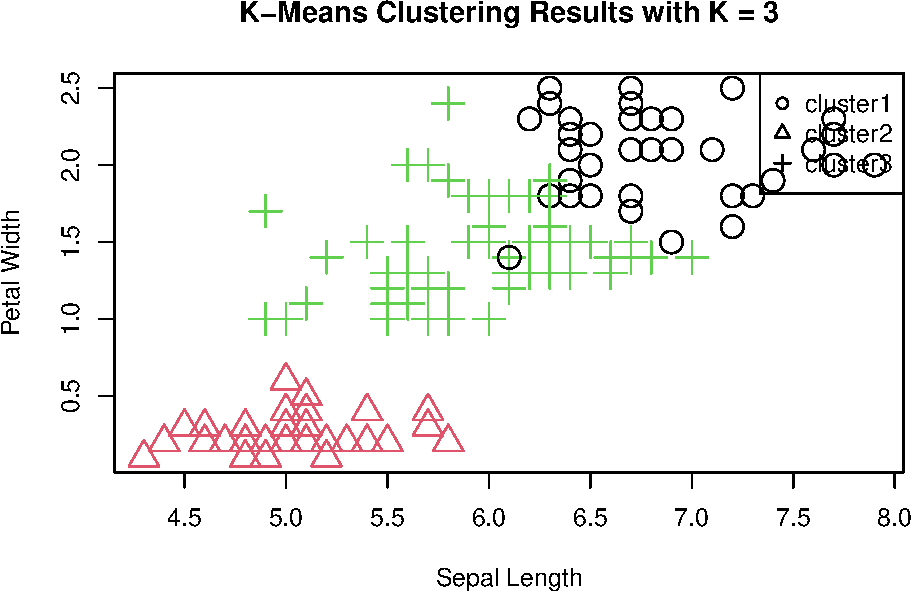
\includegraphics{189FinalProject_files/figure-latex/unnamed-chunk-3-1.pdf}

\hypertarget{c-let-beta_1-and-beta_2-be-the-coefficients-for-compprice-and-income-respectively.-test-the-hypothesis-that-ux3b21ux3b220.-state-your-hypothesis-test-statistic-and-test-statistics-distribution-clearly.-choose-an-ux3b1-you-feel-is-appropriate.}{%
\subparagraph{\texorpdfstring{(c) Let \(beta_1\) and \(beta_2\) be the
coefficients for CompPrice and Income, respectively. Test the hypothesis
that β1=β2=0. State your hypothesis, test statistic, and test
statistic's distribution clearly. Choose an α you feel is
appropriate.}{(c) Let beta\_1 and beta\_2 be the coefficients for CompPrice and Income, respectively. Test the hypothesis that β1=β2=0. State your hypothesis, test statistic, and test statistic's distribution clearly. Choose an α you feel is appropriate.}}\label{c-let-beta_1-and-beta_2-be-the-coefficients-for-compprice-and-income-respectively.-test-the-hypothesis-that-ux3b21ux3b220.-state-your-hypothesis-test-statistic-and-test-statistics-distribution-clearly.-choose-an-ux3b1-you-feel-is-appropriate.}}

\hypertarget{consider-the-carseats-data-again.}{%
\paragraph{2. Consider the Carseats data
again.}\label{consider-the-carseats-data-again.}}

\hypertarget{a-split-the-data-into-a-training-set-and-a-validation-set.-state-the-proportions-of-your-trainingvalidation-split.}{%
\subparagraph{(a) Split the data into a training set and a validation
set. State the proportions of your training/validation
split.}\label{a-split-the-data-into-a-training-set-and-a-validation-set.-state-the-proportions-of-your-trainingvalidation-split.}}

\hypertarget{bfit-a-ridge-regression-model-on-the-training-data-choosing-the-ux3bb-by-cross-validation-and-reporting-the-final-coefficients.-choose-an-appropriate-value-for-k-when-doing-cross-validation.}{%
\subparagraph{(b)Fit a ridge regression model on the training data,
choosing the λ by cross-validation and reporting the final coefficients.
Choose an appropriate value for K when doing
cross-validation.}\label{bfit-a-ridge-regression-model-on-the-training-data-choosing-the-ux3bb-by-cross-validation-and-reporting-the-final-coefficients.-choose-an-appropriate-value-for-k-when-doing-cross-validation.}}

\hypertarget{c-report-the-rmse-using-the-validation-set-on-the-model-from-2b.}{%
\subparagraph{(c) Report the RMSE using the validation set on the model
from
2b.}\label{c-report-the-rmse-using-the-validation-set-on-the-model-from-2b.}}

\hypertarget{d-fit-a-random-forest-model-on-the-training-data-and-report-the-rmse-on-the-validation-set.}{%
\subparagraph{(d) Fit a random forest model on the training data, and
report the RMSE on the validation
set.}\label{d-fit-a-random-forest-model-on-the-training-data-and-report-the-rmse-on-the-validation-set.}}

\hypertarget{efor-both-of-the-models-you-fit-in-b-and-d-give-an-example-why-a-marketing-team-would-prefer-one-model-over-the-other.}{%
\subparagraph{(e)For both of the models you fit in (b) and (d), give an
example why a marketing team would prefer one model over the
other.}\label{efor-both-of-the-models-you-fit-in-b-and-d-give-an-example-why-a-marketing-team-would-prefer-one-model-over-the-other.}}

\hypertarget{in-this-question-you-will-simulate-data-to-perform-regression-between-x-and-y.}{%
\paragraph{3. In this question, you will simulate data to perform
regression between X and
Y.}\label{in-this-question-you-will-simulate-data-to-perform-regression-between-x-and-y.}}

\hypertarget{a-use-the-rt-function-to-generate-a-predictor-x-of-length-n200.-set-df15-for-x}{%
\subparagraph{(a) Use the rt() function to generate a predictor X of
length n=200. Set df=15 for
X}\label{a-use-the-rt-function-to-generate-a-predictor-x-of-length-n200.-set-df15-for-x}}

\hypertarget{b-use-rt-to-generate-a-noise-vector-ux3f5.-set-df5.}{%
\subparagraph{(b) Use rt() to generate a noise vector ϵ. Set
df=5.}\label{b-use-rt-to-generate-a-noise-vector-ux3f5.-set-df5.}}

\hypertarget{c-generate-a-response-vector-yof-length-n-according-toy52sinx7exp2cosx1exp2cosxux3f5}{%
\subparagraph{(c) Generate a response vector Yof length n according
to:Y=5+2sin(X)−7×exp(2×cos(X))1+exp(2×cos(X))+ϵ}\label{c-generate-a-response-vector-yof-length-n-according-toy52sinx7exp2cosx1exp2cosxux3f5}}

\hypertarget{d-fit-polynomial-regression-for-y-on-x-with-the-order-of-x-ranging-from-1-to-5.-i.e.yux3b20ux3b21xux3f5yux3b20ux3b21xux3b22x2ux3f5yux3b20ux3b21xux3b22x2ux3b23x3ux3b24x4ux3b25x5ux3f5-and-plot-each-of-the-five-model-fits-in-different-colors-and-with-a-legend-on-top-of-your-simulated-data.}{%
\subparagraph{(d) Fit polynomial regression for Y on X with the order of
X ranging from 1 to 5.
(i.e.Y=β0+β1X+ϵ,Y=β0+β1X+β2X2+ϵ,\ldots,Y=β0+β1X+β2X2β3X3+β4X4+β5X5+ϵ)
and plot each of the five model fits, in different colors and with a
legend, on top of your simulated
data.}\label{d-fit-polynomial-regression-for-y-on-x-with-the-order-of-x-ranging-from-1-to-5.-i.e.yux3b20ux3b21xux3f5yux3b20ux3b21xux3b22x2ux3f5yux3b20ux3b21xux3b22x2ux3b23x3ux3b24x4ux3b25x5ux3f5-and-plot-each-of-the-five-model-fits-in-different-colors-and-with-a-legend-on-top-of-your-simulated-data.}}

\hypertarget{e-which-one-of-these-models-do-you-prefer-justify-your-answer.}{%
\subparagraph{(e) Which one of these models do you prefer? Justify your
answer.}\label{e-which-one-of-these-models-do-you-prefer-justify-your-answer.}}

\hypertarget{f-for-the-model-yux3b20ux3b21xux3b22x2ux3f5-compute-a-90-confidence-interval-at-x1-using-least-squares-theory.-provide-an-interpretation-for-this-interval.}{%
\subparagraph{(f) For the model Y=β0+β1X+β2X2+ϵ, compute a 90\%
confidence interval at X=1 using least squares theory. Provide an
interpretation for this
interval.}\label{f-for-the-model-yux3b20ux3b21xux3b22x2ux3f5-compute-a-90-confidence-interval-at-x1-using-least-squares-theory.-provide-an-interpretation-for-this-interval.}}

\hypertarget{g-for-the-model-yux3b20ux3b21xux3b22x2ux3f5-compute-a-90-confidence-interval-at-x1-using-a-bootstrap.-provide-an-interpretation-for-this-interval.}{%
\subparagraph{(g) For the model Y=β0+β1X+β2X2+ϵ, compute a 90\%
confidence interval at X=1 using a bootstrap. Provide an interpretation
for this
interval.}\label{g-for-the-model-yux3b20ux3b21xux3b22x2ux3f5-compute-a-90-confidence-interval-at-x1-using-a-bootstrap.-provide-an-interpretation-for-this-interval.}}

\hypertarget{consider-the-college-data-set-in-the-islr2-package.}{%
\paragraph{4. Consider the College data set in the ISLR2
package.}\label{consider-the-college-data-set-in-the-islr2-package.}}

\hypertarget{a-split-the-data-set-into-a-training-and-validation-set.}{%
\subparagraph{(a) Split the data set into a training and validation
set.}\label{a-split-the-data-set-into-a-training-and-validation-set.}}

\begin{Shaded}
\begin{Highlighting}[]
\FunctionTok{data}\NormalTok{(}\StringTok{"College"}\NormalTok{)}
\end{Highlighting}
\end{Shaded}

\hypertarget{b-perform-logistic-regression-on-the-training-data-to-predict-the-variable-private-using-all-other-variables.-provide-an-interpretation-of-the-coefficient-for-top10perc.}{%
\subparagraph{(b) Perform logistic regression on the training data to
predict the variable Private using all other variables. Provide an
interpretation of the coefficient for
Top10Perc.}\label{b-perform-logistic-regression-on-the-training-data-to-predict-the-variable-private-using-all-other-variables.-provide-an-interpretation-of-the-coefficient-for-top10perc.}}

\hypertarget{c-what-is-the-test-error-for-the-logistic-regression-justify-your-selection-of-your-threshold}{%
\subparagraph{(c) What is the test error for the logistic regression
(justify your selection of your
threshold)?}\label{c-what-is-the-test-error-for-the-logistic-regression-justify-your-selection-of-your-threshold}}

\hypertarget{d-fit-an-lda-to-the-same-model-and-report-the-test-error.}{%
\subparagraph{(d) Fit an LDA to the same model, and report the test
error.}\label{d-fit-an-lda-to-the-same-model-and-report-the-test-error.}}

\hypertarget{e-fit-an-qda-to-the-same-model-and-report-the-test-error.}{%
\subparagraph{(e) Fit an QDA to the same model, and report the test
error.}\label{e-fit-an-qda-to-the-same-model-and-report-the-test-error.}}

\hypertarget{f-fit-an-svm-to-the-same-model-and-report-the-test-error.}{%
\subparagraph{(f) Fit an SVM to the same model, and report the test
error.}\label{f-fit-an-svm-to-the-same-model-and-report-the-test-error.}}

\hypertarget{g-pick-which-model-you-think-is-the-best-and-explain-your-choice.}{%
\subparagraph{(g) Pick which model you think is the best and explain
your
choice.}\label{g-pick-which-model-you-think-is-the-best-and-explain-your-choice.}}

\hypertarget{for-this-problem-use-the-protein.csv-file-which-contains-protein-consumption-in-twenty-five-european-countries-for-nine-food-groups.-it-is-available-in-the-multbiplotr-r-package.}{%
\paragraph{5. For this problem use the protein.csv file which contains
protein consumption in twenty-five European countries for nine food
groups. It is available in the MultBiplotR R
package.}\label{for-this-problem-use-the-protein.csv-file-which-contains-protein-consumption-in-twenty-five-european-countries-for-nine-food-groups.-it-is-available-in-the-multbiplotr-r-package.}}

\hypertarget{a-perform-principal-component-analysis-on-these-data-omitting-variables-comunist-and-region.-report-the-proportion-of-variance-and-cumulative-proportion-of-variance-explained-by-the-first-5-principal-components.}{%
\subparagraph{(a) Perform principal component analysis on these data
(omitting variables Comunist and Region). Report the proportion of
variance and cumulative proportion of variance explained by the first 5
principal
components.}\label{a-perform-principal-component-analysis-on-these-data-omitting-variables-comunist-and-region.-report-the-proportion-of-variance-and-cumulative-proportion-of-variance-explained-by-the-first-5-principal-components.}}

\hypertarget{b-provide-an-interpretation-of-the-first-two-principal-components.}{%
\subparagraph{(b) Provide an interpretation of the first two principal
components.}\label{b-provide-an-interpretation-of-the-first-two-principal-components.}}

\hypertarget{c-create-a-biplot-for-the-first-two-principal-components.-based-on-this-plot-which-variables-is-milk-most-correlated-with-which-variables-is-milk-most-negatively-correlated-with-which-variables-is-milk-uncorrelated-with}{%
\subparagraph{(c) Create a biplot for the first two principal
components. Based on this plot, which variable(s) is Milk most
correlated with? Which variable(s) is Milk most negatively correlated
with? Which variables is Milk uncorrelated
with?}\label{c-create-a-biplot-for-the-first-two-principal-components.-based-on-this-plot-which-variables-is-milk-most-correlated-with-which-variables-is-milk-most-negatively-correlated-with-which-variables-is-milk-uncorrelated-with}}

\hypertarget{d-comment-on-the-differences-between-countries-in-the-north-region-and-central-region-using-only-the-first-two-principal-components-and-the-respective-interpretations-of-those-principal-components.}{%
\subparagraph{(d) Comment on the differences between countries in the
North Region and Central Region using only the first two principal
components and the respective interpretations of those principal
components.}\label{d-comment-on-the-differences-between-countries-in-the-north-region-and-central-region-using-only-the-first-two-principal-components-and-the-respective-interpretations-of-those-principal-components.}}

\hypertarget{conceptual-problems}{%
\subsubsection{Conceptual Problems}\label{conceptual-problems}}

\hypertarget{explain-why-the-bootstrap-may-be-more-beneficial-for-random-forest-than-it-would-be-for-linear-regression.}{%
\paragraph{6. Explain why the bootstrap may be more beneficial for
random forest than it would be for linear
regression.}\label{explain-why-the-bootstrap-may-be-more-beneficial-for-random-forest-than-it-would-be-for-linear-regression.}}

\hypertarget{give-an-example-of-a-scenario-where-you-test-multiple-hypotheses-but-would-not-want-to-corect-for-fewr-or-fdr.}{%
\paragraph{7. Give an example of a scenario where you test multiple
hypotheses but would not want to corect for FEWR or
FDR.}\label{give-an-example-of-a-scenario-where-you-test-multiple-hypotheses-but-would-not-want-to-corect-for-fewr-or-fdr.}}

\hypertarget{why-is-it-necessary-to-be-aware-of-a-models-assumptions-and-check-those-assumptions-before-using-the-trained-model-for-inference-or-prediction}{%
\paragraph{8. Why is it necessary to be aware of a model's assumptions,
and check those assumptions before using the trained model for inference
or
prediction?}\label{why-is-it-necessary-to-be-aware-of-a-models-assumptions-and-check-those-assumptions-before-using-the-trained-model-for-inference-or-prediction}}

\end{document}
